%!TEX root = Slic3r-Manual.tex
\section{Travailler avec les modèles 3D}
\label{sub:working_with_models}
\index{models}
\index{modèles 3D}

Il reste encore une étape avant la prmière impression: obtenir un modèle 3D et le "trancher".

\subsection{Formats de Modèles 3D} % (fold)
\label{sub:model_formats}
\index{STL}
\index{AMF}
\index{OBJ}

Slic3r accepte les types de fichiers suivants.

\begin{itemize}
	\item Les fichiers STéréolithographique (STL) peuvent provenir d'une grande variété de sources et sont maintenant un standard de facto dans l'impression 3D. Les fichiers décrivent simplement la géométrie de la surface d'un objet 3D sans aucune information supplémentaire (comme la couleur ou la matière), et c'est cette simplicité qui a probablement fait le format omniprésent.
	\item Le type de fichier Wavefront OBJ est un format ouvert utilisé à l'origine dans une application d'animation de Wavefront Technologies, mais a depuis été adoptée par la communauté de la modélisation 3D. Il est similaire au format STL.
	\item Le format de fichier AMF (Additive Manufacturing File Format) a été développé en réponse au caractère limité du format STL. En plus de décrire la géométrie du modèle 3D, il peut également décrire les couleurs et les matériaux, ainsi que des attributs plus complexes, tels que les mélanges dégradé et de multiples arrangements d'objets (constellations). Alors que le format est considéré comme un standard, il reste à être largement adoptée dans le milieu de la machine 3D.
\end{itemize}
% subsection model_formats (end)

\subsection{Trouver des Modèles 3D} % (fold)
\label{sub:finding_models}
\index{models!finding}
\index{modèles!trouver}

Les fichiers de modèle 3D peuvent provenir d'un dépôt en ligne, tels que Thingiverse\footnote{\url{http://www.thingiverse.com}} ou GrabCAD\footnote{\url{http://grabcad.com}}, ou être créée à partir d'un programme de CAO, comme FreeCAD\footnote{\url{http://sourceforge.net/projects/free-cad}}, Sketchup\footnote{\url{http://www.sketchup.com}}, ou OpenSCAD\footnote{\url{http://www.openscad.org}}, ou un outil de CAO en ligne tels que Shapesmith\footnote{\url{http://shapesmith.net}}.

Vous souhaitez peut-être afficher les fichiers avant de trancher et il ya beaucoup d'applications disponibles, dont l'un est Meshlab\footnote{\url{http://www.meshlab.org}} - un outil complet pour la visualisation et la manipulation des fichiers 3D.

\begin{figure}[H]
\centering
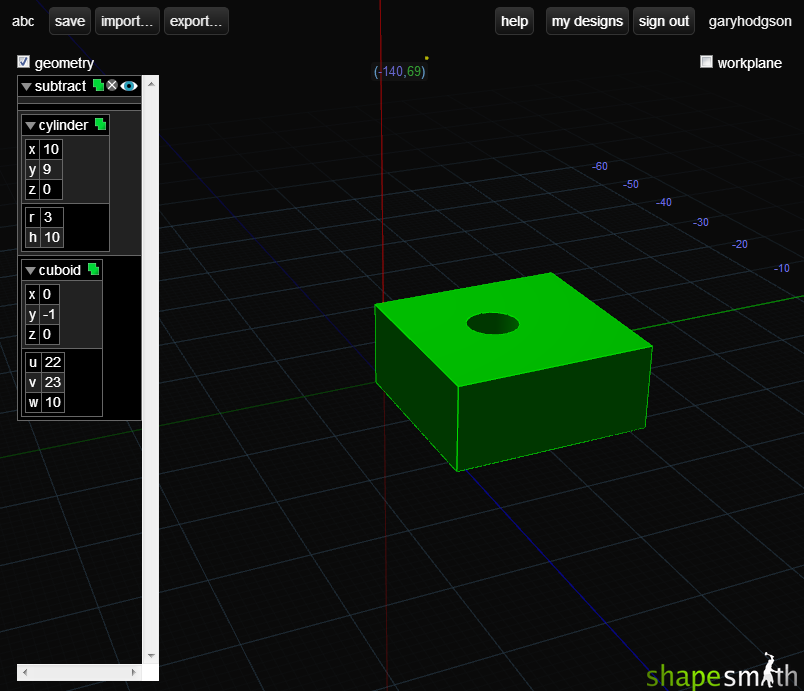
\includegraphics[keepaspectratio=true,width=0.75\textwidth]{working_with_models/shapesmith.png}
\caption{Outil de CAO en ligne Shapesmith.}
\label{fig:shapesmith}
\end{figure}

% subsection working_with_models (end)


\subsection{Utiliser la Surface de Travail} % (fold)
\label{sub:working_with_plater}
\index{Plater}
\index{Surface de Travail}
Slic3r dispose d'un outil, appelé Plater, qui permet à un ou plusieurs modèles à être chargés et disposés avant d'être "tranchés".

\begin{figure}[H]
\centering
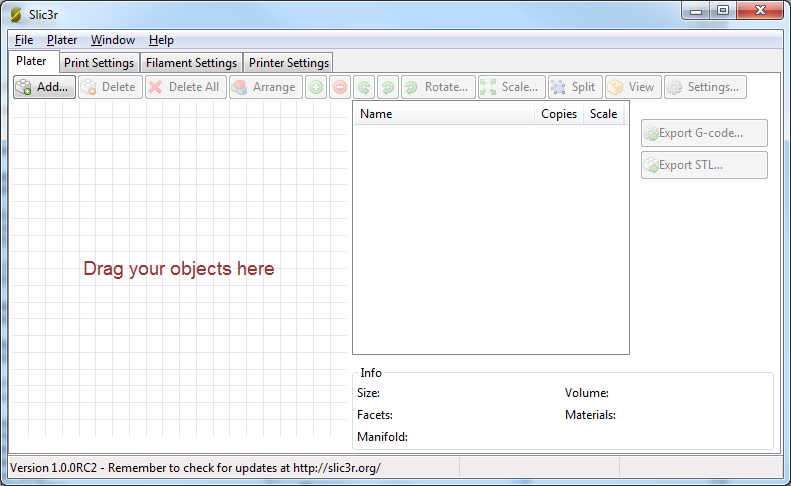
\includegraphics[keepaspectratio=true,width=1\textwidth]{working_with_models/plater.png}
\caption{Surface de Travail}
\label{fig:plater}
\end{figure}


Une fois que vous avez acquis un modèle, faites-le glisser sur l'onglet "Plater" (ou utilisez le bouton Add(Ajouter) dans le coin suppérieur gauche) pour le charger dans Slic3r. Dans la figure ci-dessous, la traditionnelle RepRap Minimug\footnote{\url{http://www.thingiverse.com/thing:18357}} is loaded, and is viewed from above. The ring around the model is a skirt - a single perimeter, several millimeters away from the model, which is extruded first.  This is useful in making sure the plastic is flowing smoothly from the nozzle when the model is starting to be printed.

\begin{figure}[H]
\centering
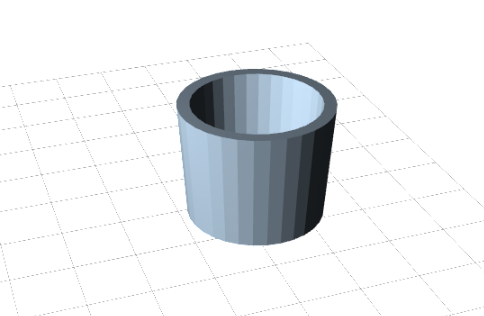
\includegraphics[keepaspectratio=true,width=0.75\textwidth]{working_with_models/minimug_model.png}
\caption{Le Modèle Minimug.}
\label{fig:minimug_model}
\end{figure}

\begin{figure}[H]
\centering
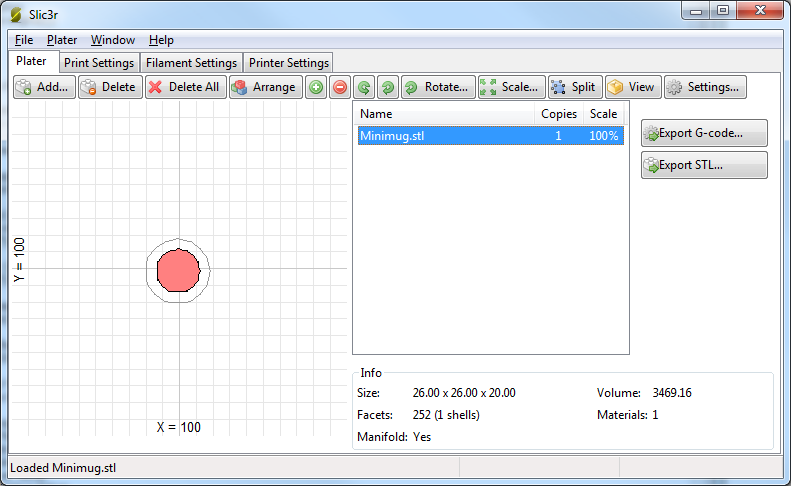
\includegraphics[keepaspectratio=true,width=1\textwidth]{working_with_models/plater_model_loaded.png}
\caption{Fichier STL chargé.}
\label{fig:plater_model_loaded}
\end{figure}

Le modèle peut être repositionnée en le déplaçant sur la reprèsentation du lit à gauche de l'écran. Notez que les dimensions du lit doivent correspondre à votre imprimante, tel qu'elles sont données lors de la configuration initiale ci-dessus.

Sur le côté droit il y a la liste des fichiers actuellement chargés. Les boutons situés en haut de la liste de fichier vous permettent d'organiser les modèles.
\begin{itemize}
	\item \textbf{More/Less (plus/moins)}  - Régle le nombre de copies qui doit être imprimé.
	\item \textbf{45°/Rotate (45°/rotation)}  - Fait pivoter le modèle sélectionné autour de l'axe Z, soit de 45 ° dans le sens horaire ou anti-horaire, ou par une valeur donnée.
	\item \textbf{Scale (échelle)}  - Augmenter ou diminuer la taille du modèle imprimé.
	\item \textbf{Split (dissocier)}  - Divise un modèle qui se compose de plus d'une partie en ses parties constituantes, ce qui permet à chacune d'être agencée individuellement.
\end{itemize}


Les boutons en haut à gauche, vous permettent d'ajouter, de supprimer, d'auto-organiser, ou d'exporter les modèles.
\begin{itemize}
	\item \textbf{Add (Ajouter)}  - Ouvre une boîte de dialogue pour ajouter un modèle à la surface de travail, c'est une alternative glissé/déposé du fichier sur la surface de travail.
	\item \textbf{Delete/Delete All (Supprimer/Tout supprimer)}  - Retirer un ou tous les modèles de la surface de travail.
	\item \textbf{Autoarrange}  - Essaye d'organiser les modèles pour obtenir l'agencement optimal.
	\item \textbf{Export G-code}  - Démarre le "tranchage" du modèle, et produit un fichier G-code.
	\item \textbf{Export STL}  - Sauvegarde un ensemble de modèle de la surface de travail dans un fichier STL unique.
\end{itemize}


% subsection working_with_plater (end)

\subsection{Réparer les fichiers STL} % (fold)
\label{sub:cleaning_stls}
\index{STL!cleaning}
\index{STL!réparer}
Si le maillage 3D décrit dans le modèle contient des trous, ou les bords ne sont pas alignés (connu comme étant non-manifold), puis Slic3r peut avoir des problèmes pour le traiter. Slic3r va tenter de résoudre les problèmesqu'il peut, mais certains problèmes sont hors de sa portée. Si l'application se plaint que le modèle ne peut pas être "tranché" correctement alors il ya plusieurs options possibles: voir le chapitre sur la Réparation des modèles.

% subsection cleaning_stls (end)